\documentclass[conference,harvard,brazil,english]{sbatex}
\usepackage[utf8]{inputenc}
\usepackage{lmodern}
\usepackage{amsmath}
\usepackage{graphicx}
\usepackage{float}

\begin{document}

\title{Controle de Temperatura de uma Torneira Elétrica}

% authors only; addresses and emails have been removed from the class
\author{Eduardo Henrique Basilio de Carvalho}
\author{Joao Vitor Braga da Silva Alves}
\author{Renan Neves da Silva}

\maketitle

\selectlanguage{brazil}

\section{Introdução}

O objetivo deste trabalho é alcançar o controle de temperatura de uma torneira elétrica sob as seguintes condições:

\begin{itemize}
    \item \textbf{Atuador:} Atuação térmica via resistências elétricas com limite de dissipação de 400 W \cite{evangelista2009plataforma}.
    \item \textbf{Elemento primário:} Transdução de temperatura via termistor NTC em topologia de Ponte de Wheatstone \cite{evangelista2009plataforma} ou sensor integrado linear LM35 \cite{mesquita_roteiro4B2,mesquita_roteiro4A1}.
    \item \textbf{Placa de aquisição:} Interface digital/analógica utilizando o modelo NI PCI-6221 (16 bits) \cite{evangelista2009plataforma} ou NI PCIe-6321 \cite{mesquita_roteiro4A4,mesquita_roteiro4B1,mesquita_roteiro4A1}.
    \item \textbf{Tiristor:} Modulação de potência elétrica imposta por TRIAC operando em regime tiristorizado governado pela variação do ângulo de disparo ($\theta$), induzindo não-linearidade estática \cite{evangelista2009plataforma,mesquita_roteiro4B2,mesquita_roteiro4A1}.
    \item \textbf{Processador:} Arquitetura x86 com processador INTEL Dual Core E2.140 operando à frequência de 1,6 GHz \cite{evangelista2009plataforma}.
    \item \textbf{Memória do computador:} Capacidade física alocada de 1 GB de memória RAM \cite{evangelista2009plataforma}.
    \item \textbf{Sistema operacional:} Distribuição Linux Ubuntu operando em \textit{user-space} \cite{evangelista2009plataforma}, estendida para suportar execução em tempo real \cite{mesquita_roteiro4A4}.
    \item \textbf{Kernel:} Núcleo Linux \textit{vanilla} submetido à camada \textit{Hardware Abstraction Layer} via \textit{patch} RTAI \cite{evangelista2009plataforma}, ou modificado para preempção integral da quase totalidade dos processos via PREEMPT\_RT \cite{mesquita_roteiro4A4,mesquita_roteiro4B1,mesquita_roteiro4A1}.
    \item \textbf{Bibliotecas:} Dependências de \textit{software} \texttt{Comedilib} e \texttt{Kcomedilib} para E/S em tempo real \cite{evangelista2009plataforma} e a API do \textit{driver} \texttt{NIDAQmx} para abstração de comunicação com o \textit{hardware} de aquisição \cite{mesquita_roteiro4A4}.
    \item \textbf{Critérios de aceitação:} Validação de estabilidade frente a perturbações em degrau de $1^{\circ}C$, avaliada tanto no centro quanto nos extremos da faixa de operação do atuador térmico \cite{mesquita_roteiro4A5e6}. O determinismo temporal do laço de controle requer a mitigação de latências, quantificadas por meio da mediana das amostras e do desvio absoluto mediano (MAD) \cite{mesquita_roteiro4A4}, além da restrição de \textit{jitter} a 10\% e tempo de ciclo de 20 $\mu s$ \cite{evangelista2009plataforma}.
\end{itemize}

\section{Caracterização da Confiabilidade Temporal do Kernel de Tempo Real}

Para caracterizar a confiabilidade temporal do kernel de tempo real, o seguinte experimento foi conduzido para $P_\text{configurado} \in \{1,10,100\}\,\text{ms}$:

\begin{enumerate}
    \item Uma quantidade $N$ de amostras é definida;
    \item Tarefas em nível de usuário e cíclicas são lançadas. Tais tarefas exercitam carga no tanto no processador quanto no sistema de E/S, este por meio de operações de leitura e escrita em arquivos;
    \item A função \texttt{DAQmxWaitForNextSampleClock} é invocada em um loop no processo principal, na função \texttt{main}, $N$ vezes;
    \item Um arranjo de períodos é coletado, no qual cada elemento $P_i$ representa o tempo decorrido entre duas invocações consecutivas da função de espera.
    \item A média $\bar{P} = \frac{1}{N} \sum_{i=1}^N P_i$ e o desvio padrão $\sigma_P = \sqrt{\frac{1}{N - 1} \sum_{i=1}^N (P_i - \bar{P})^2}$ são calculados e reportados.
\end{enumerate}

Pela limitação de recursos computacionais, o número de amostras $N$ foi definido como $N = 1000$ para $P_\text{configurado} = 1,\ 10\, \text{ms}$ e $N = 100$ para $P_\text{configurado} = 100\,\text{ms}$.

\begin{table}[H]
    \centering
    \begin{tabular}{r r r}
        \hline
        $P_\text{configurado}\ \text{ms}$ & $\bar{P}\ \text{ms}$ & $\sigma_P\ \text{ms}$ \\
        \hline
        1                                 & 1.00                 & 0.01                  \\
        10                                & 10.00                & 0.02                  \\
        100                               & 100.00               & 0.02                  \\
        \hline
    \end{tabular}
    \caption{Resultados dos experimentos de caracterização temporal do kernel de tempo real.}
    \label{tab:resultados_temporais}
\end{table}

A tabela \ref{tab:resultados_temporais} apresenta os resultados dos experimentos de caracterização temporal do kernel de tempo real. Observa-se que a média dos períodos medidos $\bar{P}$ é, nos algarismo significativos considerados, igual ao período configurado $P_\text{configurado}$ para todas as configurações testadas. O desvio padrão $\sigma_P$ é relativamente baixo, indicando que os períodos medidos estão próximos da média, o que sugere um comportamento temporal consistente do kernel de tempo real sob as condições do experimento.

\section{Coleta dos Dados}

O experimento consiste em um par de degraus, separados por tempo o suficiente para que o sistema atinja um estado estacionário, e com direções opostas. O período de amostragem selecionado é de $100 ms$. Sob este, o primeiro degrau, de $8 V$ para $2 V$, é aplicado na amostra $k = 1800$, e o segundo degrau, de $2 V$ para $8 V$, é aplicado na amostra $k = 3600$. O experimento é conduzido por um total de $N = 5400$ amostras, o que corresponde a um tempo total de aquisição de $540 s$.

As curvas levantadas são apresentadas na figura \ref{fig:experimento}.

\begin{figure}[H]
    \centering
    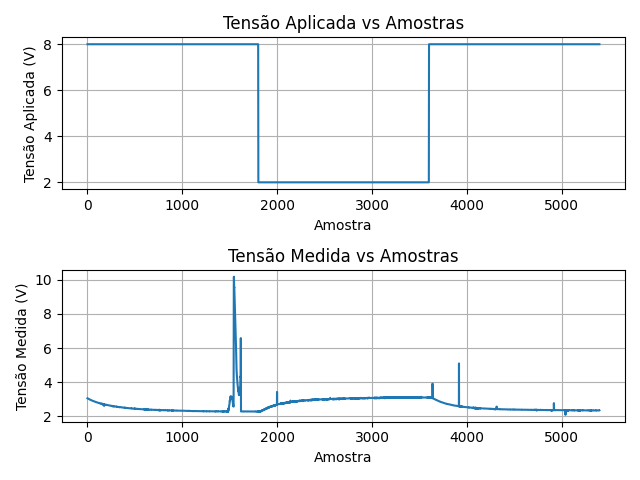
\includegraphics[width=0.75\linewidth]{../identificacao/experimento.png}
    \caption{Curvas de resposta do sistema à aplicação dos degraus.}
    \label{fig:experimento}
\end{figure}

A visualização das curvas expõe a presença de ruído e de fortes pertubações pontuais. Para a continuídade da análise, as primeiras 1620 amostras são descartadas. As curvas resultantes são apresentadas na figura \ref{fig:experimento_valido}.

\begin{figure}[H]
    \centering
    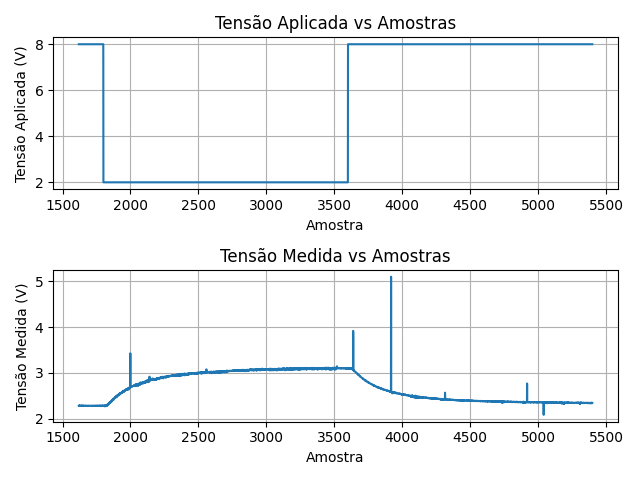
\includegraphics[width=0.75\linewidth]{../identificacao/experimento_valido.png}
    \caption{Curvas de resposta do sistema à aplicação dos degraus, após descarte das amostras iniciais.}
    \label{fig:experimento_valido}
\end{figure}

\section{Identificação do Sistema}

Dada a baixa persistencia de excitação dinâmica, percebida nos longos intervalos em que o sistema fica próximo do estado estacionário, estimadores estatísticos, como o método dos mínimos quadrados e suas variações, não são adequados para a identificação do sistema a partir deste experimento \cite{Aguirre2007}. Por isso, um modelo em função de transferência é escolhido.

O trecho de curva correspondente ao primeiro degrau, entre as amostras $k = 1620$ e $k = 3500$, é utilizado para a identificação do modelo. A figura \ref{fig:experimento_ajuste} apresenta a curva nesta faixa.

\begin{figure}[H]
    \centering
    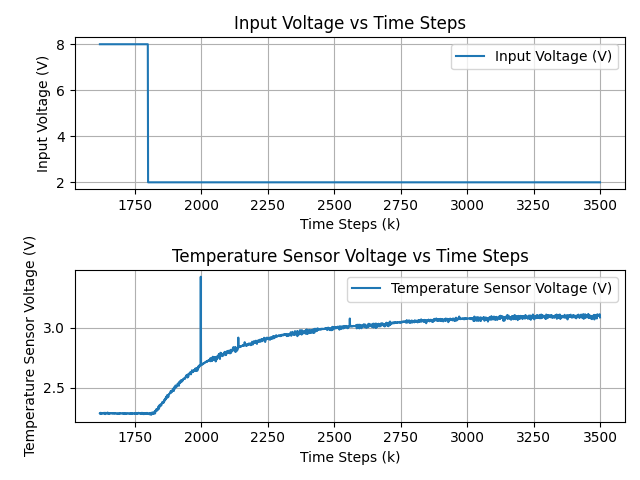
\includegraphics[width=0.75\linewidth]{../identificacao/experimento_ajuste.png}
    \caption{Curva de resposta do sistema à aplicação do primeiro degrau, entre as amostras $k = 1620$ e $k = 3500$.}
    \label{fig:experimento_ajuste}
\end{figure}

Pelas características físicas do sistema, é entendido que a dinâmica térmica da água é dominada pela dinâmica do sensor, ambas de primeira ordem. Assim, o modelo escolhido é o de um sistema de primeira ordem com atraso, cuja função de transferência é dada pela equação \ref{eq:fopdt_symbolic}.:

\begin{equation}
    G(s) = \frac{K e^{-L s}}{\tau s + 1},
    \label{eq:fopdt_symbolic}
\end{equation}

A identificação dos parâmetros é feita a partir de um processo de otimização \cite{2020SciPy-NMeth} para o qual os parametros iniciais são dados pela análise da amplitude de regime permanente, da constante de tempo e do atraso, conforme \cite{ogata2010modern}. O modelo identificado é dado pela equação \ref{eq:fopdt_identificado} e a curva anotada pelos parametros identificados é apresentada na figura \ref{fig:tempos_modelo_tf}.

\begin{equation}
    G(s) = \frac{-0.134 e^{-1.043 s}}{29.050 s + 1}.
    \label{eq:fopdt_identificado}
\end{equation}

\begin{figure}[H]
    \centering
    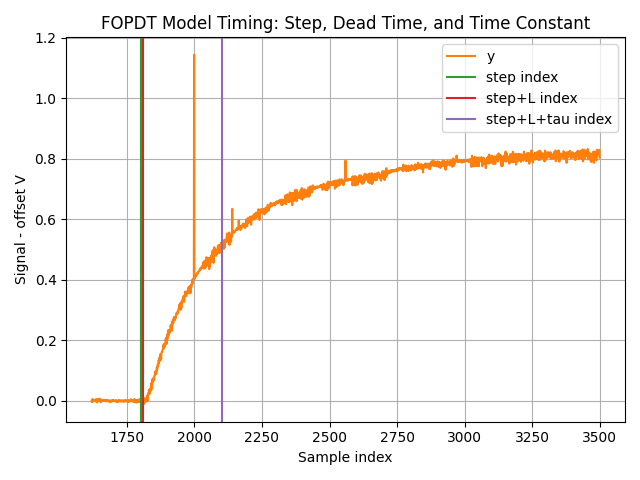
\includegraphics[width=0.75\linewidth]{../identificacao/tempos_modelo_tf.png}
    \caption{Curva de resposta do sistema à aplicação do primeiro degrau, entre as amostras $k = 1620$ e $k = 3500$, anotada pelos parâmetros identificados.}
    \label{fig:tempos_modelo_tf}
\end{figure}

A validação do modelo é feita a partir da comparação entre a curva de resposta do sistema e a curva de resposta do modelo ao segundo degrau, entre as amostras $k = 3600$ e $k = 5400$. A figura \ref{fig:predicoes_modelo_tf_teste} apresenta a curva de resposta do modelo sobreposta à curva de resposta do sistema nesta faixa. A simulação é feita em \textit{free-run}, sem alimentação com medidas do sistema, além da condição inicial.

\begin{figure}[H]
    \centering
    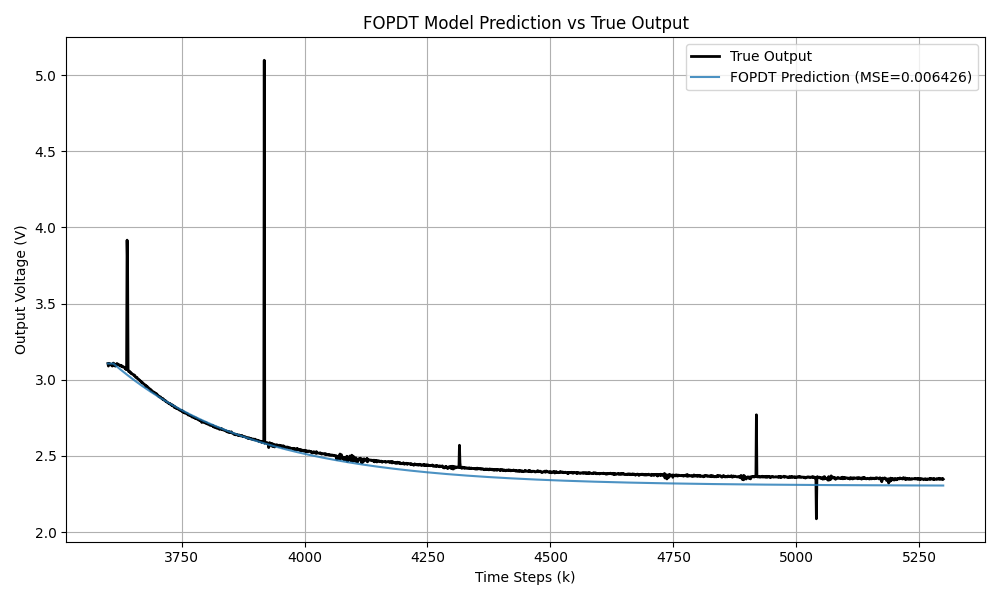
\includegraphics[width=0.75\linewidth]{../identificacao/predicoes_modelo_tf_teste.png}
    \caption{Curva de resposta do modelo sobreposta à curva de resposta do sistema, entre as amostras $k = 3600$ e $k = 5400$.}
    \label{fig:predicoes_modelo_tf_teste}
\end{figure}

Pela similaridade entre as curvas, o modelo é considerado válido para representar a dinâmica do sistema. O erro quadrático médio (MSE) entre as curvas é de $0.006$, suficientemente baixo.

\section{Projeto do Filtro Digital}

\bibliography{bibliografia}

\end{document}
